\section{Dataset}
\label{sec:dataset}

In this section, we describe the data collection process and 
the overview of the collected dataset. 


\begin{figure*}[t]
\centering
% 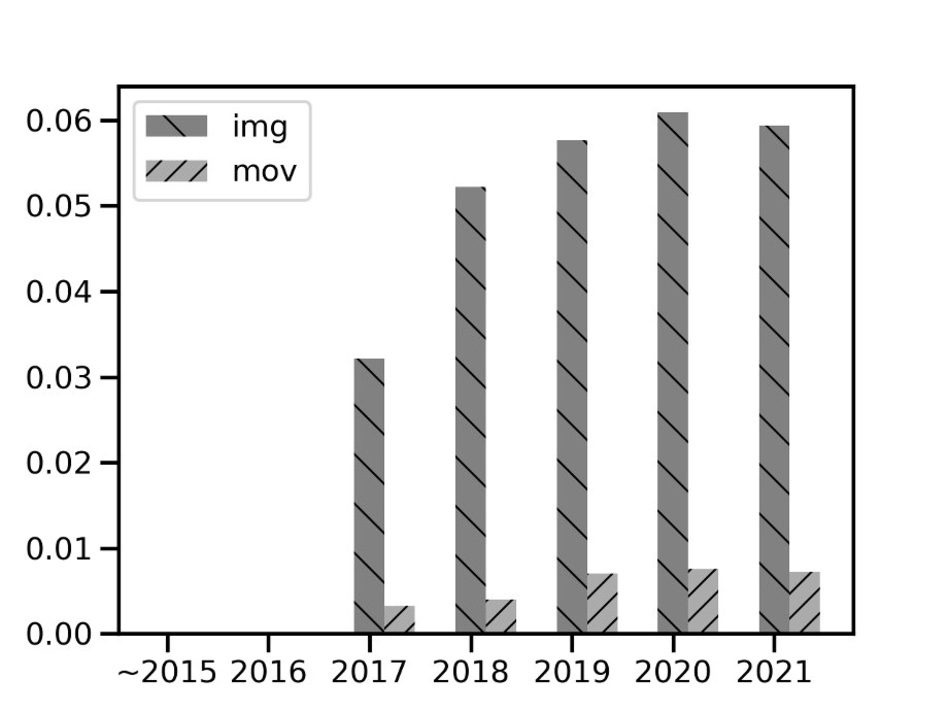
\includegraphics[width=1\linewidth]{./figures/data-category-trend.pdf}
\caption{ 
  An overview of the data collection
  }
\label{fig:data-collection-overview}
\end{figure*}


\subsection{Data Collection}
\fig{fig:data-collection-overview} shows
an overview of the data collection process.
We collected the data from the issues of 
the publicly available repositories on GitHub. 
We first select the repositories based on the following conditions:
\begin{itemize}
	\item the number of stars $\geq$ 10
	\item the number of issues $\geq$ 1
	\item the latest commit\masa{or the latest issue?} is in 2021
\end{itemize}
We used the number of stars for retrieving the repositories 
in which the owner may communicate with other developers and 
discard repositories developed by only the owner. 
In addition, we used the date of the latest commit 
because the major release of the feature is in 2021. 
Beforehand, the feature was the beta version. 
The number of the repositories that meet 
the conditions is 289,115. 
We randomly selected 4,173 repositories from them 
due to the execution time to collect issues. 
This number is less than 2\% of all repositories. 
However, the number of resolved issues 
in these repositories is already 770,656. 
We discuss the threat to validity of 
this process in \sec{sec:limitation}. 
This process was conducted from November 2021 to December 2021.


\begin{table}[t]
    \begin{center}
    \caption{The attributes we collected from the issues}
    \scalebox{0.85}[0.85]{
    \begin{tabular}{ll} 
        \toprule
        \multicolumn{1}{c}{\textbf{Attributes}} & \multicolumn{1}{c}{\textbf{Description}} \\ 
        \midrule
        $IssueResolvedTime$ & The time until the issue is resolved (day) \\
        $FirstCommentTime$ & The time until the first comment (day) \\
        $\#comments$ & The number of comments \\
        $\#chars$ & \masa{im not sure what is this} \\
        $\#imgs$ & \# of attached images when the issue is created \\
        $\#movs$ & \# of attached movies when the issue is created \\
        $\#words$ &  \masa{im not sure what is this} \\
        $IssueCreatedYear$ & The year when the issue is created \\
        \bottomrule
    \end{tabular}
    }
    \label{tab:issue-attr}
    \end{center}
\end{table}


We retrieved the attributes from the collected issues 
that are the data in the database. 
\tab{tab:issue-attr} shows the eight attributes 
retrieved from the issues. 

We used \texttt{PyGitHub}\masa{add citation} to execute GitHub API 
to retrieve the attributes from the issues. 
$IssueOpenTime$, $FirstCommentTime$,
and $IssueCreatedYear$ can be directly
retrieved by \texttt{PyGitHub}.
On the contrary,
$\#chars$, $\#imgs$, $\#movs$, and $\#words$
need the conversion from the retrieved raw data.
We describe the details of the conversion. 
The attached images and movies are transformed into 
URLs and put in the text of issues as the markdown format. 
The following URL is an example.

\begin{quote}
	https://user-images.githubusercontent.com/XXX.mp4
\end{quote}

\noindent{}
The part of XXX consists of alphanumeric, ``/'', and ``-''.
Hence, we prepared the regular expression for this URL and 
count the appearances of images and movies as $\#imgs$ and $\#movs$. 
The identification of images and movies is based on the extension of 
the URLs. 

\masa{@kuramoto: Do you remove the issues that do not have URLs?
otherwise, the following explanation is wrong}
For the issues that include the URL, we excluded them and 
counted the number of words as $\#words$. 
In addition, we counted the number of characters as $\#chars$. 

We noticed that some $IssueOpenTime$ values are less than zero. 
We decided that these values are invalid and the issues having 
these values are excluded from the dataset. 
Specifically, we only retrieved the issues that meet 
the condition: $30\ sec \leq IssueOpenTime \leq 1\ year$.
The number of issues that meet this condition is 711,160 (92.23\%).


\begin{table}[h]
    \begin{center}
    \caption{The number of issues for each category}
    \begin{tabular}{llr}
        \toprule
         & \multicolumn{1}{c}{\textbf{Description}} & \multicolumn{1}{c}{\textbf{\#issues}} \\
        \midrule
        $Img$  & $\#imgs \geq 1$ & 33,079 (4.65\%)\\
        $Mov$  & $\#movs \geq 1$ & 3,819 (0.54\%)\\
        $None$ & Others & 674,793 (94.81\%)\\ 
        \bottomrule
    \end{tabular}
    \label{classify_result}
    \end{center}
\end{table}


We classified the issues into three categories based on 
whether they have images and movies. 
\tab{tab:issue-category} shows the number of issues for each category. 
It should be noted that issues that have both 
the images and movies are counted for both 
$Img$ and $Mov$ categories. 

\begin{table*}[h]
    \begin{center}
    \caption{Examples of the retrieved issues with the values of the attributes}
    \begin{tabular}{c c c c c c c} 
      \toprule
      \textbf{IssueCreatedYear} &
      \textbf{ResolutionTime} &
      \textbf{Images} &
      \textbf{Videos} &
      \textbf{Comments} &
      \textbf{FirstCommentTime} &
      \textbf{DescriptionLength} \\
      \midrule
      2020 & 6.99861111 & 0 & 0 & 1 & 6.99861111 & 4430\\
      2020 & 41.9594329 & 1 & 0 & 3 & 17.7784722 & 85\\
      2020 & 43.8850579 & 0 & 0 & 2 & 0.49828704 & 56\\
      2020 & 44.0935532 & 0 & 0 & 4 & 0.91277778 & 33\\
      2020 & 0.14934028 & 0 & 0 & 8 & 0.08077546 & 244\\
      2020 & 59.5670949 & 2 & 0 & 5 & 0.39472222 & 102\\
      2020 & 74.9322569 & 0 & 0 & 0 & -          & 24\\
      \bottomrule
    \end{tabular}
    \label{tab:example-dataset}
    \end{center}
  \end{table*}


We extract a part of the retrieved issues in \tab{tab:example-dataset}. 
Each row corresponds to the values of the attributes of an issue. 

\begin{table}[t]
  \begin{center}
  \caption{The top-10 TFIDF words for each category}
  \begin{tabular}{l | c c c }
    \toprule
    & $Img$ & $Mov$ & $None$\\
    \midrule
    1 & image & when & dependabot\\
    2 & screenshot & dropdown & code\\
    3 & when & view & file\\
    4 & error & package & pullrequest\\
    5 & screen & issue & version\\
    6 & version & python & error\\
    7 & shot & height & use\\
    8 & file & react & lib\\
    9 & test & button & add\\
    10& code & text & commit\\
    \bottomrule
  \end{tabular}\\
  \label{tag:tfidf}
  \end{center}
\end{table}


We used $Words$ to compute the TFIDF values\masa{need citation} for each category. 
The TFIDF values will support researchers who investigate 
the differences in the appearances of words with and without 
images/movies. 
\tab{tag:tfidf} shows the top-10 TFIDF words in $Words$ 
for each category extracted from our dataset. 

\subsection{Dataset Description}

\begin{figure}[h]
\centering
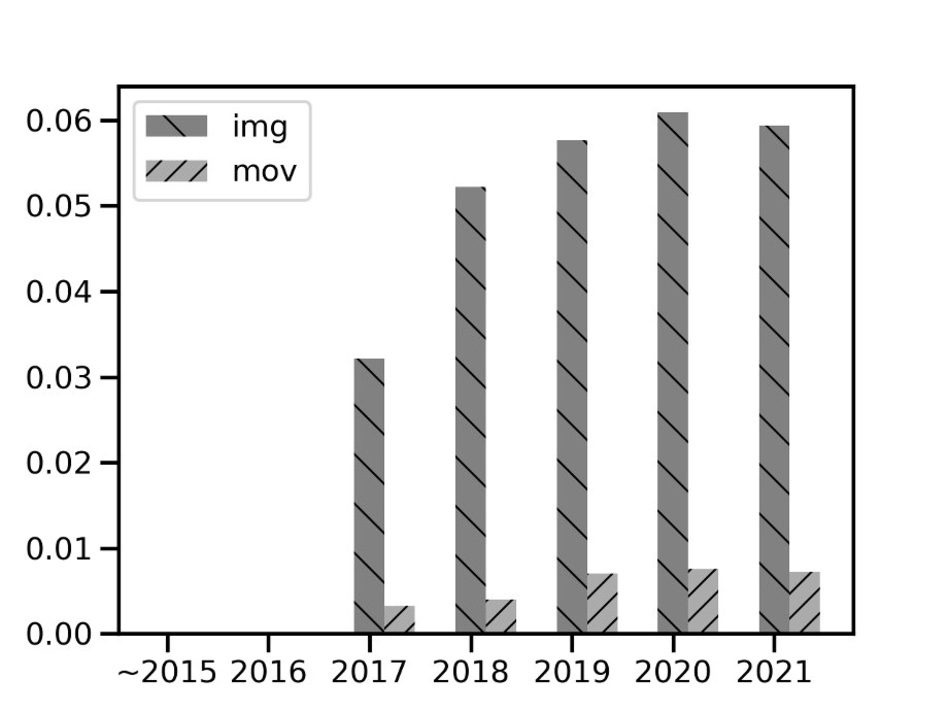
\includegraphics[width=0.6\linewidth]{./figures/data-category-trend.pdf}
\caption{ 
  The proportions of issue reports for each category
  }
\label{fig:data-cat-trend}
\end{figure}

\fig{fig:data-cat-trend} shows the proportions of 
issues in which developers attach either 
images or movies for each year. 
The y-axis shows the proportion. 
The proportions have slightly increased so far 
except for 2021. 
This may be because we collected the resolved issues 
in 2021. 
Given this result, both the images and movies are still 
not popular for developers. 


\begin{table*}[t]
  \begin{center}
  \caption{The statistics of the collected issues for each category \masa{finally we should remove this table}}
  % \scalebox{0.85}[0.85]{
  \begin{tabular}{l c c c| c c c| c c c| c c c} 
    \toprule
    & \multicolumn{3}{c}{$ResolutionTime$} & \multicolumn{3}{c}{$FirstCommentTime$} & \multicolumn{3}{c}{$Comments$} & \multicolumn{3}{c}{$DescriptionLengths$}\\
    & \textbf{$Img$} & \textbf{$Vid$} & \textbf{$None$} & \textbf{$Img$} & \textbf{$Vid$} & \textbf{$None$} & \textbf{$Img$} & \textbf{$Vid$} & \textbf{$None$} & \textbf{$Img$} & \textbf{$VId$} & \textbf{$None$} \\ 
    \midrule
    Mean & 32.60 & 40.66   & 40.01   & 8.679 & 14.83 & 13.08 &  3.556 & 3.347 & 3.262 &  104.0 & 104.3 & 149.0 \\
    Min  &       &         &         &       &       &       &        &       &       &        &       &   \\
    25th &       &         &         &       &       &       &        &       &       &        &       &   \\
    50th & 4.784 & 5.698   & 5.946   & 0.239 & 0.395 & 0.318 &  2     & 2     & 2     & 42     & 55    & 60 \\
    75th &       &         &         &       &       &       &        &       &       &  &     & \\
    Max  &       &         &         &       &       &       &        &       &       &  &  &  \\
    S.D. & 63.7  & 76.6    & 72.5    & 32.14 & 48.15 & 41.74 &  4.575 & 4.001 & 5.060 & 431.0 & 202.2 & 592.7 \\
    \bottomrule
  \end{tabular}
  % }
  \label{tab:issue_stat_categories}
  \end{center}
\end{table*}


\tab{tab:issue_stat_categories} shows the statistics
of the collected issues for the $Img$, $Mov$,
and $None$ categories.
The Mean row indicates the average values; 
the Min and Max rows indicate the minimum and maximum values; 
the 25th, 50th, and 75th rows indicate the percentile values; 
the S.D. row indicates the standard deviation values. 
We may not find the general conclusion; 
however, we observed differences across the categories. 
For example, the 25th, 50th, and 75th percentiles of 
the $Img$ and $Mov$ categories in $IssueResolvedTime$ are 
longer than those of the $None$ category. 
